\documentclass[12pt, A4]{report}

\usepackage[utf8]{inputenc}
\usepackage{graphicx}
\graphicspath{{./images/}}

\usepackage{listings}
\usepackage{xcolor}

\definecolor{codegreen}{rgb}{0,0.6,0}
\definecolor{codegray}{rgb}{0.5,0.5,0.5}
\definecolor{codepurple}{rgb}{0.58,0,0.82}
\definecolor{backcolour}{rgb}{0.95,0.95,0.92}

\lstdefinestyle{mystyle}{
    backgroundcolor=\color{backcolour},   
    commentstyle=\color{codegreen},
    keywordstyle=\color{magenta},
    numberstyle=\tiny\color{codegray},
    stringstyle=\color{codepurple},
    basicstyle=\ttfamily\footnotesize,
    breakatwhitespace=false,         
    breaklines=true,                 
    captionpos=b,                    
    keepspaces=true,                 
    numbers=left,                    
    numbersep=5pt,                  
    showspaces=false,                
    showstringspaces=false,
    showtabs=false,                  
    tabsize=2
}

\lstset{style=mystyle}


\usepackage{hyperref}
\hypersetup{
	colorlinks=true,
	linkcolor=blue,
	filecolor=magenta,      
	urlcolor=cyan,
}

\urlstyle{same}


\title{\textbf{K-Nearest Neighbours}\\ \large{Supervised ML Algorithm}}
\author{Sahasra Ranjan}
\date{April 2020}

\begin{document}

\begin{titlepage}
\maketitle
\end{titlepage}

K-Nearest Neighbours is one of the most basic yet essential algorithms in Machine Learning. It has intense application in pattern recognition, data mining and intrusion detection.

\subsection*{The algorithm}
	\begin{enumerate}
		\item Load the data
		\item Initialize K
		\item For each example in data
		\begin{itemize}
			\item Calculate the distance between the query example and the current example from the data
			\item Add the distance and the index of the example to an ordered collection
		\end{itemize}
		\item Sort the collection in ascending order.
		\item Pick the first K entries from the sorted collection
		\item Get the labels of the selected K entries
		\item If regression, return the mean else if classification, return the mode of the K labels
	\end{enumerate}

\subsection*{Chosing the right value for K}
	To select the K that’s right for your data, we run the KNN algorithm several times with different values of K and choose the K that reduces the number of errors we encounter while maintaining the algorithm’s ability to accurately make predictions when it’s given data it hasn’t seen before.\\ \\
	Here are some things to keep in mind:
	\begin{enumerate}
		\item As we decrease the value of K to 1, out predictions become less stable.
		\item Inversely, as we increase the value of K, our predictions become more stable due to majority voting (up to a certain point). Eventually, increasing K will increase the error.
		\item In cases where we are taking majority vote, we usually make K an odd number to have a tiebreaker. 
	\end{enumerate}

	\subsubsection*{Advantages}
	\begin{itemize}
		\item Simple and easy to implement.
		\item No need to build a model, tune several parameters, or make additional assumptions.
		\item Versatile, can be used for classification, regresion and search as well.
	\end{itemize}

	\subsubsection*{Disadvantages}
	\begin{itemize}
		\item Slow with increase in number of examples and/or predictors.
	\end{itemize}
	
\subsection*{Applications}
	KNN’s main disadvantage of becoming significantly slower as the volume of data increases makes it an impractical choice in environments where predictions need to be made rapidly. Moreover, there are faster algorithms that can produce more accurate classification and regression results.\\ \\
	However, provided you have sufficient computing resources to speedily handle the data you are using to make predictions, KNN can still be useful in solving problems that have solutions that depend on identifying similar objects. An example of this is using the KNN algorithm in recommender systems, an application of KNN-search.

\subsection*{Implementation}
\lstinputlisting[language=Python, caption=Python Implementation for K-Nearest Neighbours Algorithm]{kNN-implementation.py}

\begin{figure}[h]
	\centering
	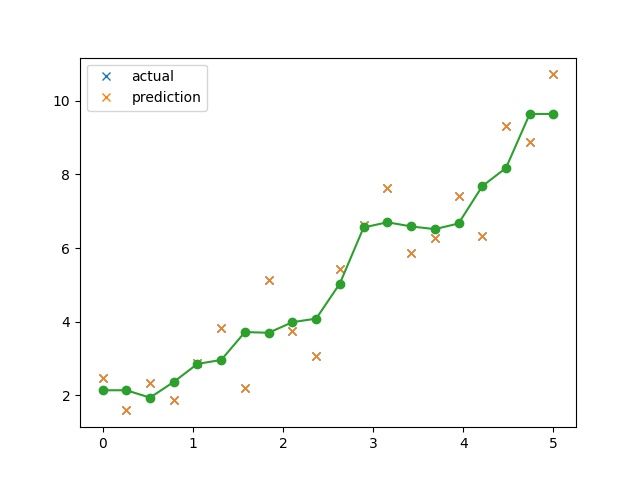
\includegraphics[scale=0.8]{kNNplot.png}
	\caption{Matplotlib plot for above implementation}
\end{figure}


\end{document}